%The Materials and Methods section provides sufficient detail for other 
%scientists to reproduce the experiments presented in the paper. In some 
%journals, this information is placed in an appendix, because it is not what 
%most readers want to know first.

% explicit preview would be phrased much like the object of the document: 
%"This section first . . . , then . . . , and finally . . . "
% Do not make readers guess: Make sure the paragraph's first sentence gives 
%them a clear idea of what the entire paragraph is about.
%%%%%%%%%%%%%%%%%%%%%%%%%%%%%%%%%%%%%%%%%%%%%%%%%%%%%%%%%%%%%%%%%%%%%%%%%%%%%%
\section{Adaptive Optics Methods applied in Microscopy}
\label{sec:ExperimentDiscussion}

Adaptive optics techniques have found their way into almost all kinds of modern, high resolution microscopy techniques. These microscopes have been combined with direct wavefront sensing and sensorless AO, using deformable mirrors or spatial light modulators for aberration compensation~(all of which has been described in Section~\ref{Measurement}. This includes standard widefield microscopes as well as highly sophisticated and specialized point scanning methods such as Coherent Antistokes Raman Spectroscopy~(CARS) and STimulated Emission Depletion~(STED) techniques. It has to be noted however, that some of these methods are themselves only a few years old. Therefor, they are still being optimized and so are the AOM techniques. It is therefore an interesting field of research with new ideas being implemented every year.\newline
AO was first used in confocal and two-photon fluorescence microscopy, both of which are commonly used in biomedical applications. These microscopes suffer from a significant drop in signal and resolution as the focus is moved deeper into the specimen, which is caused by aberrations~\cite{characterizing_abberations}.

AOM is also used for imaging of live specimens. Due to an increased excitation signal and improved light collection from the specimen, acquisition times can be reduced and contrast can be enhanced. Techniques that without AO are to slow for live imaging might now be usable, opening up completely new fields of research. Another advantage of AO lies in the microscopy design. Using AO methods, can help the designer to relax the aberration tolerance. This permits a significant reduction in the complexity of the optical system while maintaining diffraction limited operation.

This section will describe, using state of the art examples, how AO is implemented in both widefield and point scanning systems.  


%%%%%%%%%%%%%%%%%%%%%%%%%%%%%%%%%%%%%%%%%%%%%%%%%%%%%%%%%%%%%%%%%%%%%%%%%%%%%
\subsection{Widefield Microscopy}
\label{sec:WidefieldMicroscopy}

As mentioned above, AO techniques are being applied in widefield microscopy. In conventional microscopes, widefield illumination is provided using back light illumination or in the case of reflection or fluorescence modes, via the objective lens. The image quality depends only on the aberrations induced in the detection path and is independent of the aberrations of the illumination path. Aberration correction is therefore only necessary in the detection path and a single pass adaptive optics system will suffice~\cite{book_aberrations}. Hence, the goal of AO for widefield microscopy is to restore the best possible imaging and to correct for aberrations induced both by an imperfect imaging system as well as by the imaged specimen. The latter becomes more important for thick biological samples where the light has to travel a larger distance through a medium with an inhomogeneous refractive index. 

Many other highly specialized widefield microscopy techniques have been developed and for most of those, AO schemes for aberration correction and resolution optimization have been presented. Two widefield microscopye techniques will be presented in this section. First the implementation of AO in a standard transmission microscope~(Section~\ref{sec:TransmissionMicroscope}) using a sensorless wavefront sensing scheme is explained. How the theoretical background of this technique can be applied to more sophisticated microscopy schemes is then shown on the example of structured light illumination~(Section~\ref{sec:StructuredIlluminationMicroscopy}), a specialized wide field technique. 

Not covered by this report is the application of AO using a direct wavefront sensing scheme as presented by \emph{Azucena et al.} in 2011 using a Shack–Hartmann wavefront sensor, a fluorescent reference source, and a deformable mirror~\cite{wide_directSensing_microscope}. Adaptive optics can also be used to correct for aberrations in fluorescence microscopy.  There, the aberration caused by an refractive index mismatch between sample, cover plate and immersion medium can by calculated theoretically and is then corrected~\cite{wide_AOM_FM_spehrical_correction} or the aberration is measured using a guide-start technique~\cite{wide_fluorescence_guide_star} as described in Section~\ref{Measurement}. AO is also applicable in multifocal multiphoton microscopy~\cite{wide_MPFM,wide_MMM_AO}.


%------------------------------------------------------------------------------
\subsubsection{Transmission Microscope}
\label{sec:TransmissionMicroscope}
To implement adaptive optics with standard (incoherent) transmission microscopes, \emph{Debarre et al.}~\cite{wide_AOM_loew_freq} implement an indirect, sensorless and image-based adaptive optics scheme, as shown in Fig.~\ref{fig:widefield_simple_microscope}. As described earlier in Section~\ref{sec:IndirectWavefrontSensing}, image-based techniques do not require an additional wavefront sensor but retrieve the correction data directly form the recorded images. As with all indirect sensing schemes, the difficulty is to find a good metric for image quality, which allows to determine the appropriate correction parameters.

\begin{figure}[htb]
	\centering
		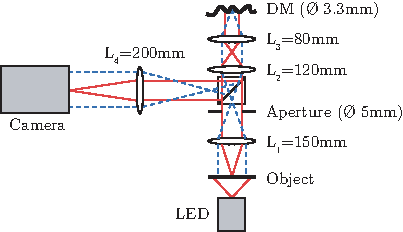
\includegraphics[width=0.50\textwidth]{images/widefield_simple_microscope.pdf}
	\caption{Schematic diagram of the experimental setup, showing a simple microscope complemented with a deformable mirror for aberration correction. Image after~\cite{wide_AOM_loew_freq}.}
	\label{fig:widefield_simple_microscope}
\end{figure}

The presented method uses low spatial frequency content of the image as the optimization metric. The aberration is represented in terms of so called Lukosz modes. Like Zernike polynomials, the Lukosz functions are each expressed as the product of a radial polynomial and an azimuthal function. The presented technique is based on modeling the effects of aberrations on the imaging of low spatial frequencies, which Lukosz modes are are found to be ideal for.

\noindent By modeling the aberration $\Phi(r)$ as a series of $N$ Lukosz modes $L_i(r,\phi)$ with coefficients $a_i$~\cite{wide_Lukosz_Modes}:
\begin{align}
	\Phi(r) = \sum_{i=4}^{N+3}{a_i L_i(r,\phi)},
	\label{eq:aberration_expansion_Lukosz}
\end{align}
they develop the optimization metric $g$ as the sum of a range of low frequencies. It is related to the coefficients of the aberration expansion, $a_i$ by the Lorentzian function~\cite{wide_AOM_loew_freq}
\begin{align}
	g(a_i) \approx \frac{1}{q_0 + q_1 \sum_{i=4}^{N+3}{a_i^2}}
	\label{eq:aberration_metric}
\end{align}
where the piston, tip and tilt modes ($i = 1,2,3$ respectively) have been omitted and $q_0$ and $q_1$ are both positive quantities in the frequency range of interest. The aberration correction process is then performed as the maximization of $g(a_i)$. Because of this particular aberration expansion and  optimization metric, the function $g(a_i)$ shows a paraboloidal maximum that permits the use of simple maximization algorithms. Furthermore, it is shown that the optimization can be performed as a sequence of independent maximizations for each aberration coefficient. 

\begin{figure}[tbh]
			\centering
			\begin{subfigure}[b]{0.8\textwidth}
							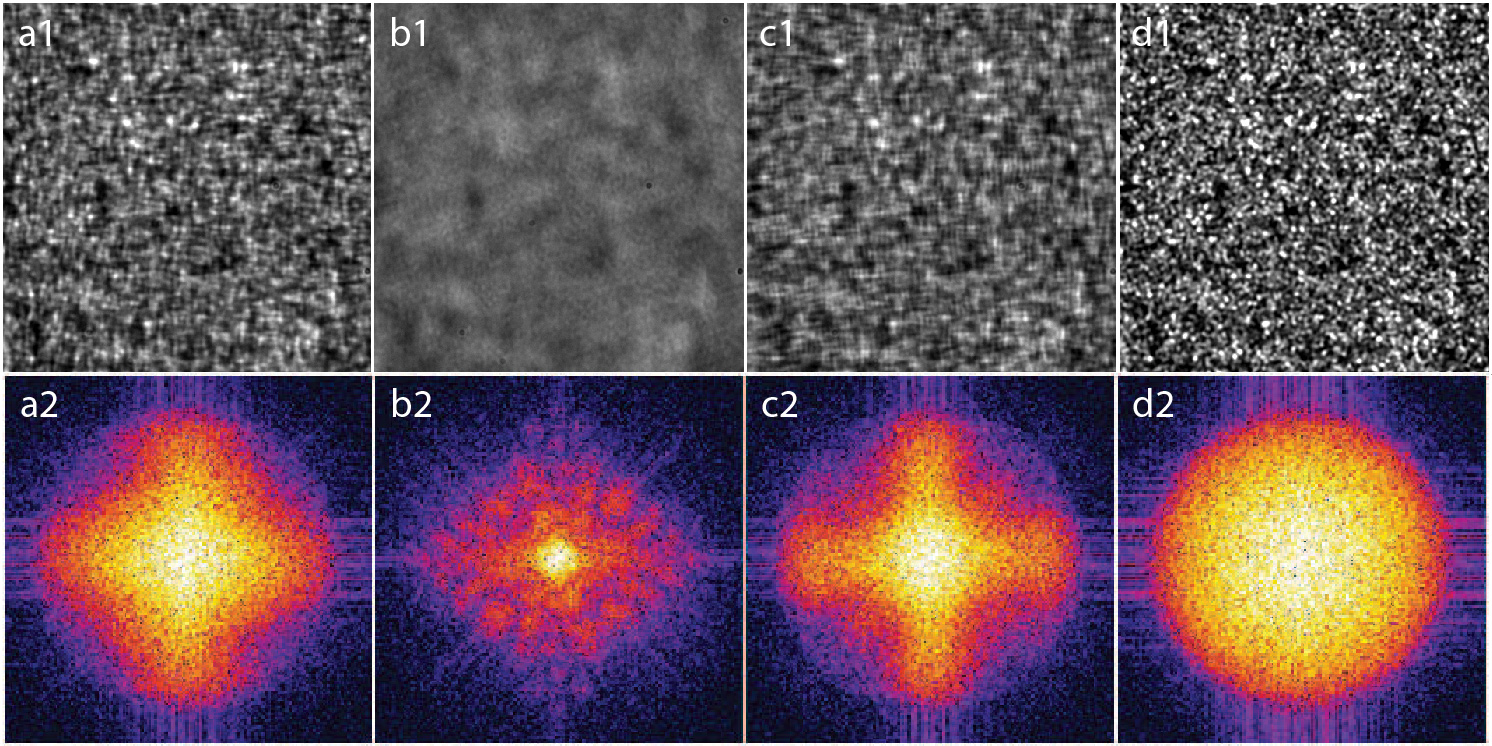
\includegraphics[width=\textwidth]{images/wide_parabolic_opti_images}
							\label{fig:para_opt_images}
			\end{subfigure}
			\begin{subfigure}[b]{0.8\textwidth}
							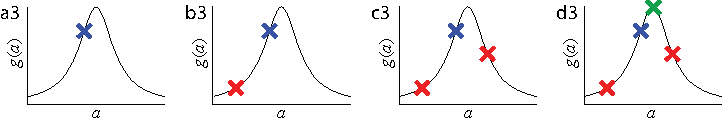
\includegraphics[width=\textwidth]{images/wide_parabolic_opti_graphs}
							\label{fig:para_opt_graphs}
			\end{subfigure}								
			\caption{Correction of a single Lukosz aberration mode (astigmatism, i = 5) for a scatterer specimen and using low spatial frequencies. The first row shows the raw images of the specimen and the second row contains the corresponding spectral densities. The third row illustrates schematically the sampling of the Lorentzian curve used in the optimization calculation. (a1-a3) correspond to an arbitrary initial aberration of magnitude, (b1-b3) have an additional negative bias while (c1-c3) have an additional positive bias of equal magnitude. (d1- d3) show the corrected image calculated with the parabolic minimizationn. Image after~\cite{wide_AOM_loew_freq}.}
	\label{fig:para_opt}
\end{figure} 

The correction process is shown in Figure~\ref{fig:para_opt} for the correction of a single Lukosz mode using a scatterer specimen. Using the deformable mirror (DM), an initial aberration $a_i$ is applied and an image is recorded. The Fourier transform and spectral density of the image are then calculated and the appropriate range of frequency components are summed, giving the metric measurements $g_0$. The same procedure is repeated with both negative and positive aberrations~(i.e. stronger and weaker aberrations), resulting in the metric measurements $g_-$ and  $g_+$. Due to the paraboilc maximum of Eq. \eqref{eq:aberration_metric}, the value of $a_i$ that minimizes $g$ can be calculated from as little as three measurements of $g(a_i)$. The optimum correction aberration can then estimated by parabolic minimization as~\cite{wide_parabolic_optimization}:
\begin{align}
	a_\text{corr} = \frac{b(g_+ - g_-)}{2g_+ - 4g_0 + 2g_-}
\end{align}
and is then applied to the DM. To correct multiple modes, each modal coefficient is measured in the same manner before the full correction aberration containing all modes is applied. While this technique is based only on low spatial frequencies, it is shown that both low and high frequency components can be effectively corrected. In all the cases investigated, a Strehl ratio greater than 0.8, close to the diffraction limit, was obtained. This indicates that, when aberration statistics are unknown, choosing small spatial frequencies for an initial correction is a reasonable strategy. If further correction is required,they can be performed using a larger range of frequencies. \emph{Debarre et al.} conclude that this correction scheme is largely independent of the object structure and propose that this approach also to be valid for coherent or partially coherent systems.


%------------------------------------------------------------------------------
\subsubsection{Structured Illumination Microscopy}
\label{sec:StructuredIlluminationMicroscopy}

It is often desired for biological samples to produce clear images of focal planes deep within a thick sample (i.e. optical sectioning) and common techniques include point-scanning techniques such as confocal or multiphoton techniques which are described in Section~\ref{sec:PointScanningMicroscopes}. 

Widefield techniques such as Structured Illumination (SI) microscopy can also provide optical sectioning. However, there the sectioning is realized using a standard microscopes, an incoherent light source and without the need for a scanning mechanism. For SI microscopy, a grid is imaged into the specimen to produce a one-dimensional sinusoidal excitation pattern in the focal plane. The resulting sinusoidal fluorescence image, consisting of both in- focus and out-of-focus fluorescence emission, is then normally recorded. Several images are taken, each corresponding to a different grid position equivalent to three different phase shifts of the grating. The grid pattern only appears in the focal plane while it is blurred in the out of focus regions. Hence, it is possible to extract an optical section from the spatially modulated component of the images via a simple calculation.

Based on the SI microscopy technique presented by \emph{Neil et al.} in 2005~\cite{wide_structured_illu_principle} as well as their earlier work on indirect wavefront sensing using a conventional microscope~\cite{wide_AOM_loew_freq} in 2007~(described in the previous section) \emph{Debarre et al.} combined both techniques in 2008 and proposed an AO scheme for use in SI microscopy~\cite{wide_AOM_structured_illu}.  

\begin{figure}
	\centering
		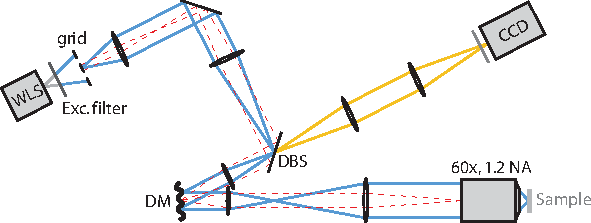
\includegraphics[width=0.75\textwidth]{images/wide_structured_illumination.pdf}
	\caption{Experimental setup for structured illumination microscopy with 
aberration correction. WLS~-~white light source, DM~-~deformable mirror, DBS
~-~dichroic beamsplitter. The blue rays mark the illumination path; the 
detection path is shown in yellow. Image after~\cite{wide_AOM_structured_illu}
.}
	\label{fig:wide_structured_illumination}
\end{figure}

They again present a sensorless wavefront detection scheme, which is shown in Fig.~\ref{fig:wide_structured_illumination}. The method to obtain the aberration correction is similar to the one presented and explained in the previous section. 
The authors derive an inner product from a mathematical model of the imaging process, followed by an orthogonalization process applied to a set of Zernike polynomials. Based on that, a general method providing an optimal aberration expansion for the chosen optimization metric is presented. This process yields  information about the effects of different aberration modes in of the SI microscope. \emph{Debarre et al.} show that the image quality mainly depends on the imaging efficiency spatial frequency of the illumination pattern. This imaging efficiency is affected much more by some aberration modes~(called grid modes) than by others~(called non-grid modes) . Grid modes have a significant influence on the intensity of the sectioned image, whereas non-grid modes have comparatively little effect. The non-grid modes do however affect the resolution. 

The results of the implemented AO scheme is shown in Fig.~\ref{fig:structured_light_correction} for aberration correction on a fluorescent mouse intestine. The image contrast and sharpness improvement is clearly visible in image~\ref{fig:SI_corrected} compared to the uncorrected image in \ref{fig:SI_uncorrected}. As a result of the aberration correction, and as shown in Fig.~\ref{fig:SI_scan}, the contrast of small sample features (blue arrows) is better defined after (red solid line) rather than before (black dotted line) correction. 

\begin{figure}[tbh]
        \centering
        \begin{subfigure}[b]{0.25\textwidth}
                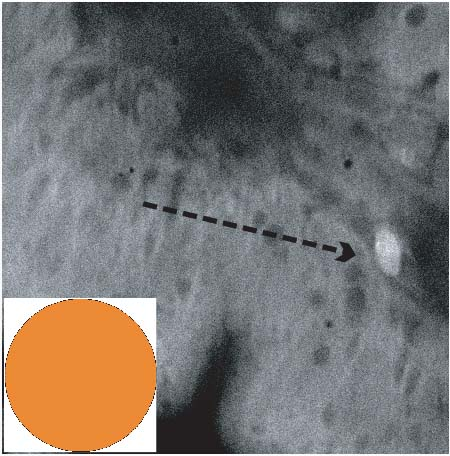
\includegraphics[width=\textwidth]{images/structured_illumination_uncorrected}
                \caption{Uncorrected.}
                \label{fig:SI_uncorrected}
        \end{subfigure}
        \begin{subfigure}[b]{0.25\textwidth}
                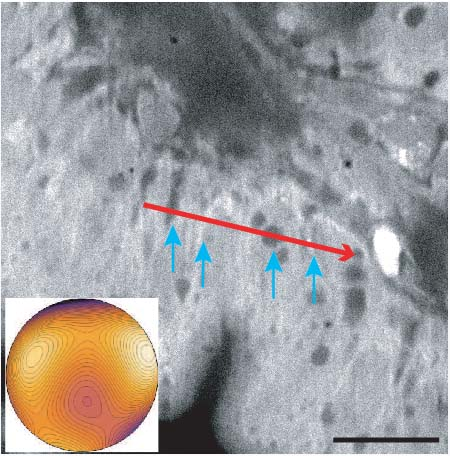
\includegraphics[width=\textwidth]{images/structured_illumination_corrected}
                \caption{Corrected.}
                \label{fig:SI_corrected}
        \end{subfigure}
        \begin{subfigure}[b]{0.25\textwidth}
                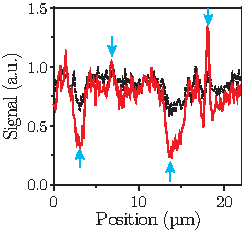
\includegraphics[width=\textwidth]{images/structured_illumination_scan}
                \caption{Line Scan.}
                \label{fig:SI_scan}
        \end{subfigure}
								
        \caption{Aberration correction in structured illumination microscopy. 
A fluorescent mouse intestine sample was imaged (a) without (b) with 
aberration correction with inserts showing the phase induced by the 
deformable mirror. (c) Profile along the lines drawn on the images, both 
profiles normalized so that their mean value is identical. As a result of the 
resolution improvement, the contrast of small sample features (blue arrows) 
is better defined after (red solid line) rather than before (black dotted 
line) correction. The imaging depth was approximately $\unit[10]{\upmu m}$, 
sacle bar size $\unit[10]{\upmu m}$. Image after~\cite{wide_AOM_structured_illu}
.}
\label{fig:structured_light_correction}
\end{figure} 

The authors also explain an additional benefit of aberration correction for structured illumination microscopy. That the adaptive element can also be used to improve the rejection of the out-of-focus fluorescence. When imaging thick specimen, noise fluctuations in the fluorescence signal between the three successive widefield images obtained for the maximization process result in a large out-of-focus background in the calculated sectioned images. Since this background arises from fluorescence generated outside the focal plane, it is not  sensitive to the presence of aberrations. By applying large aberrations in a number of grid modes, the grid pattern is suppressed and only the out-of-focus noise can be measured. By subtracting this aberrated image from the original sectioned image, the fluorescent background can be efficiently removed, leading to greatly improved contrast of the in-focus structures.

The aberrations can also change significantly with depth and hence using the same correction for different depths can result in a degradation of the image quality.  The correction can however be adapted for different imaging depths in the sample. This permits improvement of the image quality throughout an axially extended sample.
It is furthermore possible to determined the appropriate modes once and use the same scheme for any specimen, as the scheme is mostly independent of the object structure. Alternatively, if one wants to correct for local variations in aberrations the image could be formed from several sub-images for which independent aberration correction would be performed.

%TODO is this technique applied in Point Scanning Techniques? 
In conclusion, the authors present a sophisticated, easy to implement and highly versatile AOM scheme which allows for aberration correction induced by the optical system, the specimen or the focus depth. While the presented scheme uses a widefield microscope, \emph{Debarre et al.} are also optimistic that similar AO methods based on indirect, image based aberration detection can be applied to point-scanning methods. 


%------------------------------------------------------------------------------
\subsection{Point Scanning Microscopes}
\label{sec:PointScanningMicroscopes}

Just as with the widefield techniques, adaptive optics quickly found its way into point scanning techniques to improve the image and signal quality. 

Scanning methods are useful for imaging biological specimens, since they can provide high resolution imaging in three-dimensions. Illumination is  usually provided by a laser that is focused into the sample. The light emitted or reflected from the specimen is collected, usually through the same objective lens, and its intensity is measured by a detector. Since this only provides information about the intensity at a single spot, focal point is then scanned through the specimen and point-by-point the image is acquired. 

%ToDo - check what we will actually describe and write short intro for that here...
Several other point scanning microscope modalities have been introduced, including Two-Photon Excitation Fuorescence (TPEF) microscopy, second harmonic generation (SHG) and third harmonic generation (THG) microscopy, and coherent anti-Stokes Raman (CARS) microscopy.

- using a fluorescence microscope, the smaller FWHM, provided by the optimized DMM, will increase the excitation intensity leading to a higher fluorescent signal for the same laser beam input power

\cite{scan_HG_embryos,scan_HG_dynamic} -> Both the second- and third-harmonic intensity signals are used as the optimization metric
- Aberration correction is performed to compensate both system- and specimen-induced aberrations by using an efficient optimization routine based upon Zernike polynomial modes
- images of live mouse embryos show an improved signal level and resolution.
- The peak intensity increased by almost $\unit[50]{\%}$ and the FWHM decreased by $\unit[14]{\%}$ to  $\unit[1.22]{\upmu m}$ compared with a value of $\unit[1.15]{\upmu m}$ for an unaberrated system

\cite{scan_CARS} - signal improvement 3x for samples at a depth of $\unit[700]{\upmu m}$ and ~6x for muscle tissue at a depth of $\unit[260]{\upmu m}$
- completely random optimization, approach is well suited to CARS microscopy, since photobleaching does not occur 
- optimization algorithm typically converged after 3000 mirror shapes, mirror speed up to 1kHz this can be pretty fast

\cite{scan_STED} (2012) - STED principle \cite{scan_STED_principle} (1994) 
- STED phase mask as well as aberration correction realized using the SLM
- aberration correction in both depletion beam (better resolution) and in the excitation beam path (better signal and less noise)
- due to depletion image brightness as metric not good, introduced a new metric that seeks to optimize both image brightness and image sharpness in a combined approach,
- imaging through a \#1.5 coverglass ($\unit[0.15]{mm}$ thicknes) and ~$\unit[55]{\upmu m}$ glycerol, Comparing the axial profiles of the STED and AO STED reveals a \~5-fold increase in the peak signal as well as a \~3.2-fold improvement in resolution 



%------------------------------------------------------------------------------
-
\subsubsection{Confocal Microscopes}
\label{sec:ConfocalMicroscopes}

The confocal microscopy can be operated in reflection or fluorescence mode. Both are a dual pass system, which means that either the illumination path and the emission path have to be corrected in an AO confocal microscope. 

The first attempt to apply AO in confocal microscopy was done by \textit{Martin J. Booth et al.} \cite{scan_CFM}. They implemented indirect wavefront sensing to a confocal fluorescence microscope in a closed-loop way. Aberration measurement and correction was done sequentially. First a preset positive bias aberration was introduced by a deformable membrane mirror. An image scan was taken and all of its pixel values were summed and averaged to give the value of $W_1$. Then, it was added to the system the equivalent negative bias aberration, obtaining $W_2$. They had shown before that the value of the difference signal, W = $W_1$-$W_2$, is approximately proportional to the amount of the Zernike mode Zi present in the sample. They applied this procedure for several different Zernike modes, updating the mirror shape each time. A simple representation of the experimental set-up is shown in Fig.~\ref{fig:AOM_scan_CFM}.

\begin{figure}[htbp]
	\centering
		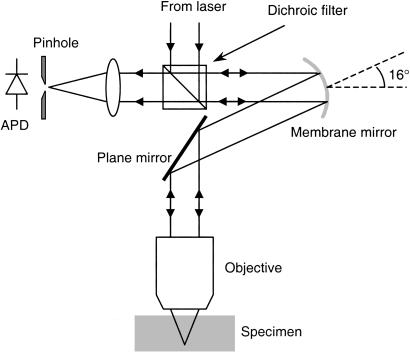
\includegraphics[width=0.42\textwidth,height=0.22\textheight]{images/AOM_scan_CFM.jpg}
		\caption{The illumination beam was passed through a beam expander and reflected by the membrane mirror such that the angle between the incident and reflected beams was 16º. Then it passed into the objective lens focusing the light into the specimen. Fluorescence light from the specimen was collected by the same objective. In this configuration, the membrane mirror can compensate for aberrations introduced into both the illumination and emission optical paths.}
	\label{fig:AOM_scan_CFM}
\end{figure}
  
With this sequential method for correcting aberrations they achieve an axial PSF shorter by a factor of 1.8, using two cycles of this modal wavefront sensor applied to low order aberration modes. Obviously, the degree of correction required and the profit of this method depend upon the nature of each individual specimen. 

Another different way to apply AO in confocal microscopy was done by \textit{Xiaodong Tao et al} \cite{scan_Confocal_direct_sensing}. They used a direct wavefront sensor in a fluorescence confocal microscope. Particularly, they implemented a Shack-Hartmann sensor with fluorescent micro-spheres (1 $\mu$ m diameter) embedded in the sample as a point source reference beacons. Their set-up was designed to operate in a close-loop. The corrector device was a deformable mirror. A separate laser channel was added to excite the microsphere, which shared the same light path with the imaging channel. The results showed a 4.3x improvement in the Strehl ratio and a 240 $\%$ improvement in the signal intensity for fixed mouse tissues at depths of up to 100 $\mu$m. Although the effects of these microspheres in the live tissue have to be further investigated, this direct method enabled a shorter exposure time during sensing and a higher speed of imaging, which showed its potential ability for live in vivo imaging.

%------------------------------------------------------------------------------
\subsubsection{Two-Photon Fluorescence Microscopy}
\label{sec:twoPhotonExcitation}

Its intrinsic optical sectioning, larger penetration depth, reduced photo damage as well as other advantages allowed nonlinear microscopy in general, and Two-Photon Fluorescence Microscopy~(TPFM) in particular, to become a very important tool in biological imaging since its first presentation by \emph{Denk et al.} in 1990~\cite{scan_TPFM_principle}. As with most AO microscopy techniques, both a direct and indirect wavefront sensing scheme can be deployed for the use with TPFM. Indirect sensing was already explained~(section~\ref{sec:IndirectWavefrontSensing}) and presented~(section~\ref{sec:WidefieldMicroscopy} in detail. \emph{Marsh et al.} present the first and fairly simple indirect sensing approach, correcting only for depth induced aberrations as early as 2003~\cite{scan_TPFM_pratical}. Again, based on their earlier works~(\cite{wide_AOM_loew_freq,wide_AOM_structured_illu}), \emph{D\'{e}barre et al.} present another highly sophisticated application of their image based wavefront sensing scheme in 2009~\cite{scan_TPFM_image_based}. Since both \emph{Marsh} and \emph{D\'{e}barre} essentially use the standard TPFM setup and the image optimization is very similar to the one presented earlier, we will not describe these methods here again. \emph{Rueckel et al.} present a wavefront correction method using coherence-gated wavefront sensing~\cite{scan_TPFM_gated_wavefront} which also beyond the scope of this report. This section will therefor describe direct wavefront sensing based on the work presented by \emph{Aviles-Espinosa et al.} in 2011~\cite{scan_TPFM_guide_start}.\newline

For two-photon fluorescence microscopy, it is not essential to correct for sample or system induced aberrations on the collected beam. Since it is a point scanning technique, all the light emitted in the focus region is collected and only the relative intensity difference is important for the generation of the image~(see \cite{scan_TPFM_review} for a detailed review on TPFM). To achieve the highest possible resolution, especially when imaging deep in a tissue, it is however very important to correct aberrations of the excitation beam. This will not only result in a better, i.e. smaller focus spot, but will also highly increase the efficiency of the nonlinear process. As described in earlier sections, a indirect wavefront sensing is usually applied for microscopic applications. While indirect sensing has several advantages over direct sensing~(see sec. \ref{sec:IndirectWavefrontSensing}), they have one important drawback that can ultimately not be overcome. They all depend on an iterative optimization procedure to estimate and correct for the aberrations. While random optimization requires many iterations~(in some cases up to 3000 iterations per mirror actuator~\cite{scan_CARS}) other methods base the iterations on complicated models and are able to achieve indirect sensing with as little as $2N+1$ iterations~(where N is the number of corrected aberration modes)~\cite{wide_AOM_loew_freq,wide_AOM_structured_illu,scan_TPFM_image_based}. However, even these methods require the sample to be exposed and imaged multiple times. To correct 11 aberrations modes (as done in~\cite{scan_TPFM_image_based}), one needs 23 exposure to acquire an aberration corrected image. While this is suitable for some systems such as CARS where photobleaching is not an issue, it often limits the feasibility of AO in florescence imaging. Being aware of these limitations, \emph{Aviles-Espinosa et al.} therefore developed a direct sensing scheme. 

As described in section~\ref{sec:WavefrontSensing}, to be able to use a wavefront sensor, one needs a point like reference source which is then used to detect the aberration. This point like source, called ``nonlinear guide star'' ``(NL-GS) by the authors\footnote{The term ``guide start'' is used in reference to astronomy. There a star or an laser spot projected in the sky is used as the reference and called guide star.}, can be artificially created and imbedded in the sample, as done for standard fluorescence microscopy~\cite{wide_fluorescence_guide_star}. This however can cause damage to the sample or might influence the behavior of living samples, limiting its potential for in vivo imaging. \emph{Aviles-Espinosa et al.} realized that two-photon excited fluorescence naturally produces a small confined volume which can be used as the guide-star. The setup presented by the authors is shown in Fig.~\ref{fig:TPFM_guide-star}. The setup shown is basically an inverted microscope, modified to be used as laser scanning TPFM (see paper for detailed component description and working principle. A mode locked Ti:sapphire laser~($\lambda = \unit[810]{nm}$ \& $\unit[860]{nm}$, pulse duration = $\unit[100]{fs}$, repetition rate = $\unit[80]{MHz}$, average powers in sample plane = $\unit[1.5]{mW}$ to $\unit[5.6]{mW}$) is used as the excitation beam. The wavefront sensing is performed using a Shack-Hartmann WaveFront Sensor (SH WFS), located at one of the output ports of the microscope. The aberration correction is realized with an electromagnetic Deformable Mirror (DM). 

\begin{figure}
	\centering
		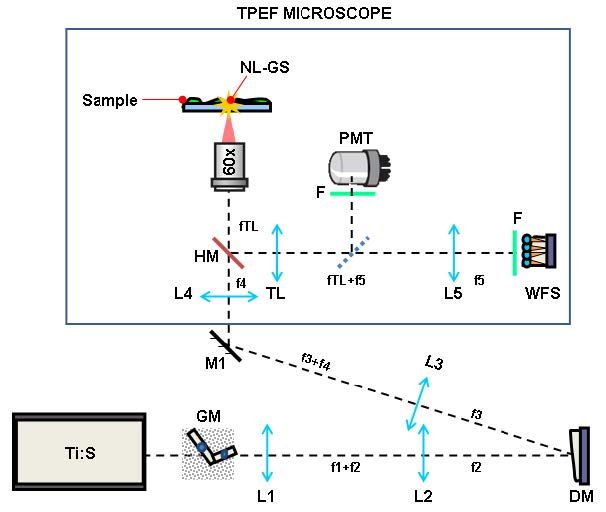
\includegraphics[width=0.75\textwidth]{images/TPFM_guide-star}
	\caption{Experimental setup for aberration corrected two-photon fluorescence microscopy as proposed by \emph{Aviles-Espinosa et al.}. GM - galvanometric mirrors, L1-L5 - lenses, DM - deformable mirror, M1 - mirror, HM - filter and beamsplitter, MO - microscope objective, TL - microscope tube lens, F - band pass filters, PMT - photo multiplier tube, WFS - Shack-Hartmann wavefront sensor. The microscope output port is manually selected either for the PMT or for the WF sensor using PS. See~\cite{scan_TPFM_guide_start} for the original image as well as a detailed description of the working principle.}
	\label{fig:TPFM_guide-star}
\end{figure}

Before the authors started their experiments on biological samples, they first showed that the guide star is reproducible, reliable and independent from the excitation beam aberrations. They continued to verify that the NL-GS behaves as point source as well as proving that aberrations are similar in the complete Field Of View (FOV). Since all these requirements were met, it was show that aberrations in the imaged area can be effectively corrected using only one NL-GS. The authors then continued to calibrate their system, eliminating the passive aberrations of the microscope system coming from the optics for excitation beam as well as the beam path from the objective pupil to the output ports of the microscope. These so called coupling aberrations only need to be corrected once for a given microscopic setup. They were measured and taken into account as a reference for all the subsequent wavefront measurements. The second correction step was to measure the so called focusing aberrations caused by the focusing part of the system. This step was performed every time prior to the actual image acquisition to account for the specific measurement~(i.e. the objective, the refractive index matching oil, the cover slip and the sample).\newline

The authors then investigated the performance of their AOM system using both Caenorhabditis elegans and mouse brain samples. -For small aberrations and weak scattering only a modest improvement in signal intensity was shown. At an imaging depth of $\unit[25]{\upmu m}$, the  measured signal enhancement was 1.75x by correcting the coupling aberrations, and 3.61x when focusing aberrations were corrected as well. Similar values were obtained imaging deeper into the tissue. 
Caenorhabditis elegans tissue scatterers only weakly and hence spherical aberration is the main aberration for imaging deep into the tissue. Since these should be easily corrected using the presented scheme, the authors were surprised by these relatively small improvements if the signal quality. By using an additional agar pad to simulate moderate scattering as well as imaging deeper into the tissue, the authors investigated the correction efficiency further. Deep in the sample~($\unit[127]{\upmu m}$) where large sample induced aberrations are prominent, improvements of the signal intensity by a factor of 22.59 were possible, as shown in Fig.~\ref{fig:elegance}. It is noteworthy, that the aberration correction increases the signals local maxima while the local minima remain unaltered. 

\begin{figure}[tbh]
			\centering
			\begin{subfigure}[b]{0.20\textwidth}
							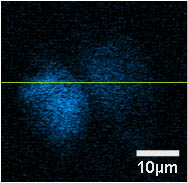
\includegraphics[width=\textwidth]{images/elegance_uncorrected}
							\caption{Uncorrected.}
							\label{fig:elegance_uncorrected}
			\end{subfigure}
			\begin{subfigure}[b]{0.20\textwidth}
							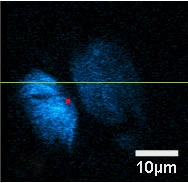
\includegraphics[width=\textwidth]{images/elegance_coupling_cor}
							\caption{Coupling cor.}
							\label{fig:elegance_coupling}
			\end{subfigure}		
			\begin{subfigure}[b]{0.20\textwidth}
							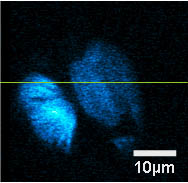
\includegraphics[width=\textwidth]{images/elegance_all_corr}
							\caption{Focusing cor.}
							\label{fig:elegance_all_corr}
			\end{subfigure}
			\begin{subfigure}[b]{0.37\textwidth}
							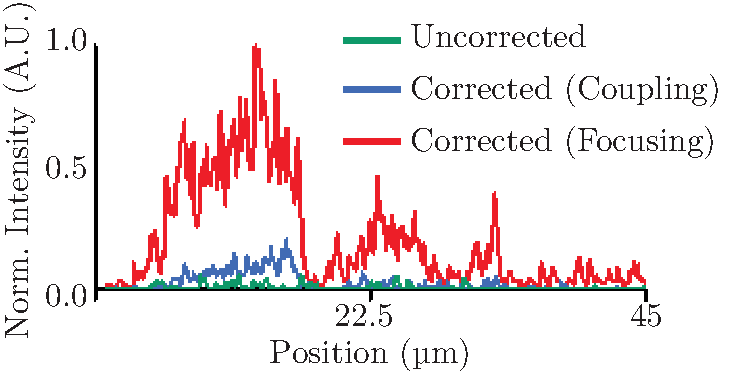
\includegraphics[width=\textwidth]{images/elegance_result}
							\caption{Line Scan.}
							\label{fig:elegance_result}
			\end{subfigure}							
			\caption{In vivo C. elegans sample imaged at $\unit[127]{\upmu m}$ depth. (a) shows the uncorrected image of a worm section, (b) displays the same section with coupling correction applied and (c) shows the section when both coupling and focusing aberrations are corrected. (d) shows the intensity profile along the green line in the images for all three correction cases. The correction of coupling aberrations improves the signal intensity by a factor of only 1.94 whereas the correction of both coupling and focusing aberrations results in a very good improvement of 22.59. Image after~\cite{scan_TPFM_guide_start}.}
	\label{fig:elegance}
\end{figure} 

Finally, the authors investigate the AO system performance using strongly scattering mouse brain tissue. They show that a correction is still possible, but it is less efficient than for moderately scattering samples. It is furthermore possible to record aberration corrected images with a single exposure, no need for complex optimization algorithms and without further sample preparation~(i.e. no fluorescent beads need to be inserted). This minimize photobleaching effects, photo-toxicity and limits negative effects to the living sample. Since no model is needed to correct the aberrations, the method is robust and can be applied to fixed and in vivo biological samples. An overall intensity improvement of more than one order of magnitude was shown is some cases. 
In conclusion, the authors present and flexible and versatile appication of adaptive optics in microscopy which can be used in wide range biological imaging applications where a high resolution is required. 

